% Texas 2015

\documentclass[10pt,a4paper]{article}\usepackage[]{graphicx}\usepackage[]{color}
%% maxwidth is the original width if it is less than linewidth
%% otherwise use linewidth (to make sure the graphics do not exceed the margin)
\makeatletter
\def\maxwidth{ %
  \ifdim\Gin@nat@width>\linewidth
    \linewidth
  \else
    \Gin@nat@width
  \fi
}
\makeatother

\definecolor{fgcolor}{rgb}{0.345, 0.345, 0.345}
\newcommand{\hlnum}[1]{\textcolor[rgb]{0.686,0.059,0.569}{#1}}%
\newcommand{\hlstr}[1]{\textcolor[rgb]{0.192,0.494,0.8}{#1}}%
\newcommand{\hlcom}[1]{\textcolor[rgb]{0.678,0.584,0.686}{\textit{#1}}}%
\newcommand{\hlopt}[1]{\textcolor[rgb]{0,0,0}{#1}}%
\newcommand{\hlstd}[1]{\textcolor[rgb]{0.345,0.345,0.345}{#1}}%
\newcommand{\hlkwa}[1]{\textcolor[rgb]{0.161,0.373,0.58}{\textbf{#1}}}%
\newcommand{\hlkwb}[1]{\textcolor[rgb]{0.69,0.353,0.396}{#1}}%
\newcommand{\hlkwc}[1]{\textcolor[rgb]{0.333,0.667,0.333}{#1}}%
\newcommand{\hlkwd}[1]{\textcolor[rgb]{0.737,0.353,0.396}{\textbf{#1}}}%

\usepackage{framed}
\makeatletter
\newenvironment{kframe}{%
 \def\at@end@of@kframe{}%
 \ifinner\ifhmode%
  \def\at@end@of@kframe{\end{minipage}}%
  \begin{minipage}{\columnwidth}%
 \fi\fi%
 \def\FrameCommand##1{\hskip\@totalleftmargin \hskip-\fboxsep
 \colorbox{shadecolor}{##1}\hskip-\fboxsep
     % There is no \\@totalrightmargin, so:
     \hskip-\linewidth \hskip-\@totalleftmargin \hskip\columnwidth}%
 \MakeFramed {\advance\hsize-\width
   \@totalleftmargin\z@ \linewidth\hsize
   \@setminipage}}%
 {\par\unskip\endMakeFramed%
 \at@end@of@kframe}
\makeatother

\definecolor{shadecolor}{rgb}{.97, .97, .97}
\definecolor{messagecolor}{rgb}{0, 0, 0}
\definecolor{warningcolor}{rgb}{1, 0, 1}
\definecolor{errorcolor}{rgb}{1, 0, 0}
\newenvironment{knitrout}{}{} % an empty environment to be redefined in TeX

\usepackage{alltt}
\usepackage[utf8]{inputenc}
\usepackage[charter]{mathdesign}
\usepackage[scaled=.95]{inconsolata}
\usepackage[margin=1.1in]{geometry}
\usepackage{color}

\usepackage{hyperref}
\usepackage{dcolumn,booktabs} %% for memisc
\usepackage{graphicx}
\usepackage{amsmath}

%\usepackage{stitchr} %% make me compile as latex when knitr is not applied

\definecolor{darkblue}{rgb}{0,0,.6} % not really
\definecolor{other}{rgb}{0,0,.5}
\hypersetup{colorlinks=true, linkcolor=darkblue, citecolor=darkblue, 
	filecolor=darkblue,urlcolor=other}

\setlength{\parskip}{1em}
\setlength{\parindent}{0em}


\author{Texas A\&M  2015}
\title{Scaling lab}
\date{}
\IfFileExists{upquote.sty}{\usepackage{upquote}}{}
\begin{document}
\maketitle


\subsection*{US Senate Speeches}

Let's take a look at US Senate debate on partial birth abortion. We want to use the speeches to estimate individual positions based on Senatorial rhetoric. 



Open $R$. Let's first start by installing and loading the package \texttt{austin} that allows us to run \textit{Wordscores} or \textit{Wordfish}: 
\begin{knitrout}
\definecolor{shadecolor}{rgb}{0.969, 0.969, 0.969}\color{fgcolor}\begin{kframe}
\begin{alltt}
\hlkwd{library}\hlstd{(austin)}
\end{alltt}


{\ttfamily\noindent\itshape\color{messagecolor}{\#\# Loading required package: numDeriv}}\end{kframe}
\end{knitrout}
If this did not work you may need to install it as follows:
\begin{knitrout}
\definecolor{shadecolor}{rgb}{0.969, 0.969, 0.969}\color{fgcolor}\begin{kframe}
\begin{alltt}
\hlkwd{install.packages}\hlstd{(}\hlstr{'austin'}\hlstd{,} \hlkwc{repos}\hlstd{=}\hlstr{"http://r-forge.r-project.org"}\hlstd{,} \hlkwc{type}\hlstd{=}\hlstr{"source"}\hlstd{)}
\end{alltt}
\end{kframe}
\end{knitrout}
Now change the working directory to the one with the csv file you just created. Now, read in the term document matrix (you might have called yours something else)
\begin{knitrout}
\definecolor{shadecolor}{rgb}{0.969, 0.969, 0.969}\color{fgcolor}\begin{kframe}
\begin{alltt}
\hlstd{data} \hlkwb{<-} \hlkwd{read.csv}\hlstd{(}\hlstr{'us-abortion-debate.csv'}\hlstd{,} \hlkwc{row.names}\hlstd{=}\hlnum{1}\hlstd{)}
\end{alltt}
\end{kframe}
\end{knitrout}

First, let's check that we have the term document matrix correctly. First we chck the dimensions
\begin{knitrout}
\definecolor{shadecolor}{rgb}{0.969, 0.969, 0.969}\color{fgcolor}\begin{kframe}
\begin{alltt}
\hlkwd{dim}\hlstd{(data)}
\end{alltt}
\begin{verbatim}
[1]   12 2705
\end{verbatim}
\end{kframe}
\end{knitrout}
The matrix should contain 12 documents (rows) and 2705 words (columns). Typing
\begin{knitrout}
\definecolor{shadecolor}{rgb}{0.969, 0.969, 0.969}\color{fgcolor}\begin{kframe}
\begin{alltt}
\hlstd{data[}\hlnum{1}\hlopt{:}\hlnum{5}\hlstd{,}\hlnum{1}\hlopt{:}\hlnum{5}\hlstd{]}
\end{alltt}
\begin{verbatim}
                  mr presid   i thank the
sessionsREP.txt    4      4  31     2 102
santorumREP.txt    3      6 102     5 574
lautenbergDEM.txt  2      5  32     2  87
hatchREP.txt       1      4  15     0  57
harkinDEM.txt      2      1  46     2 134
\end{verbatim}
\end{kframe}
\end{knitrout}
shows the first five documents and the first five words. It does indeed look like a term document matrix.

Before fitting a \texttt{Wordfish}, we need to do some final processing of this matrix. First, we will tell the program that it is a word frequency matrix with the words in columns (it could also look the other way round, that is why we need to tell the computer).  Let's write this into a new object that we call \texttt{senate}. This way, we preserve the original \texttt{data} object in the memory, in case we want to go back.
\begin{knitrout}
\definecolor{shadecolor}{rgb}{0.969, 0.969, 0.969}\color{fgcolor}\begin{kframe}
\begin{alltt}
\hlstd{senate} \hlkwb{<-} \hlkwd{wfm}\hlstd{(data,} \hlkwc{word.margin}\hlstd{=}\hlnum{2}\hlstd{)}
\end{alltt}
\end{kframe}
\end{knitrout}
Now we fit the model. Remember that the scaling procedure is completely based on differences in word frequencies and generates estimates in one dimension. We simply need to fix two documents to tell the program how it should anchor this dimension (we can always aribitrarily rotate the dimension by multiplying all estimates by $-1$). 

By default the first document will a smaller position value than the tenth document.  You can alter this by setting the \texttt{dir} parameter (see \texttt{?wordfish} for details).  
We estimate and write the output into a new object:
\begin{knitrout}
\definecolor{shadecolor}{rgb}{0.969, 0.969, 0.969}\color{fgcolor}\begin{kframe}
\begin{alltt}
\hlstd{senate.res} \hlkwb{<-} \hlkwd{wordfish}\hlstd{(senate)}
\end{alltt}
\end{kframe}
\end{knitrout}
This should take not very long to estimate. Let's take a look at the estimation results: 
\begin{knitrout}
\definecolor{shadecolor}{rgb}{0.969, 0.969, 0.969}\color{fgcolor}\begin{kframe}
\begin{alltt}
\hlkwd{summary}\hlstd{(senate.res)}
\end{alltt}
\begin{verbatim}
Call:
	wordfish(wfm = senate)

Document Positions:
                  Estimate Std. Error   Lower   Upper
sessionsREP.txt     0.5907    0.04630  0.4999  0.6814
santorumREP.txt     0.5719    0.02215  0.5285  0.6153
lautenbergDEM.txt  -0.5027    0.05817 -0.6168 -0.3887
hatchREP.txt        0.9025    0.04795  0.8085  0.9965
harkinDEM.txt      -0.5572    0.05351 -0.6621 -0.4523
feinsteinDEM.txt   -1.9309    0.01517 -1.9606 -1.9011
ensignREP.txt       0.7371    0.05458  0.6302  0.8441
durbinDEM.txt      -0.2895    0.06349 -0.4139 -0.1651
dewineREP.txt       1.1125    0.03415  1.0455  1.1794
brownbackREP.txt    1.2620    0.01972  1.2233  1.3006
boxerDEM.txt       -1.4280    0.01528 -1.4579 -1.3980
allardREP.txt      -0.3501    0.08199 -0.5108 -0.1894
\end{verbatim}
\end{kframe}
\end{knitrout}
This table shows an overview of the position estimates, the standard errors, and confidence intervals. This is hard to read, so we can plot it instead, as in Fig~\ref{senplot}.
What story do the estimates tell about the debate? 

\begin{figure}[htbp]
\begin{center}
\begin{knitrout}
\definecolor{shadecolor}{rgb}{0.969, 0.969, 0.969}\color{fgcolor}\begin{kframe}
\begin{alltt}
\hlkwd{plot}\hlstd{(senate.res)}
\end{alltt}
\end{kframe}
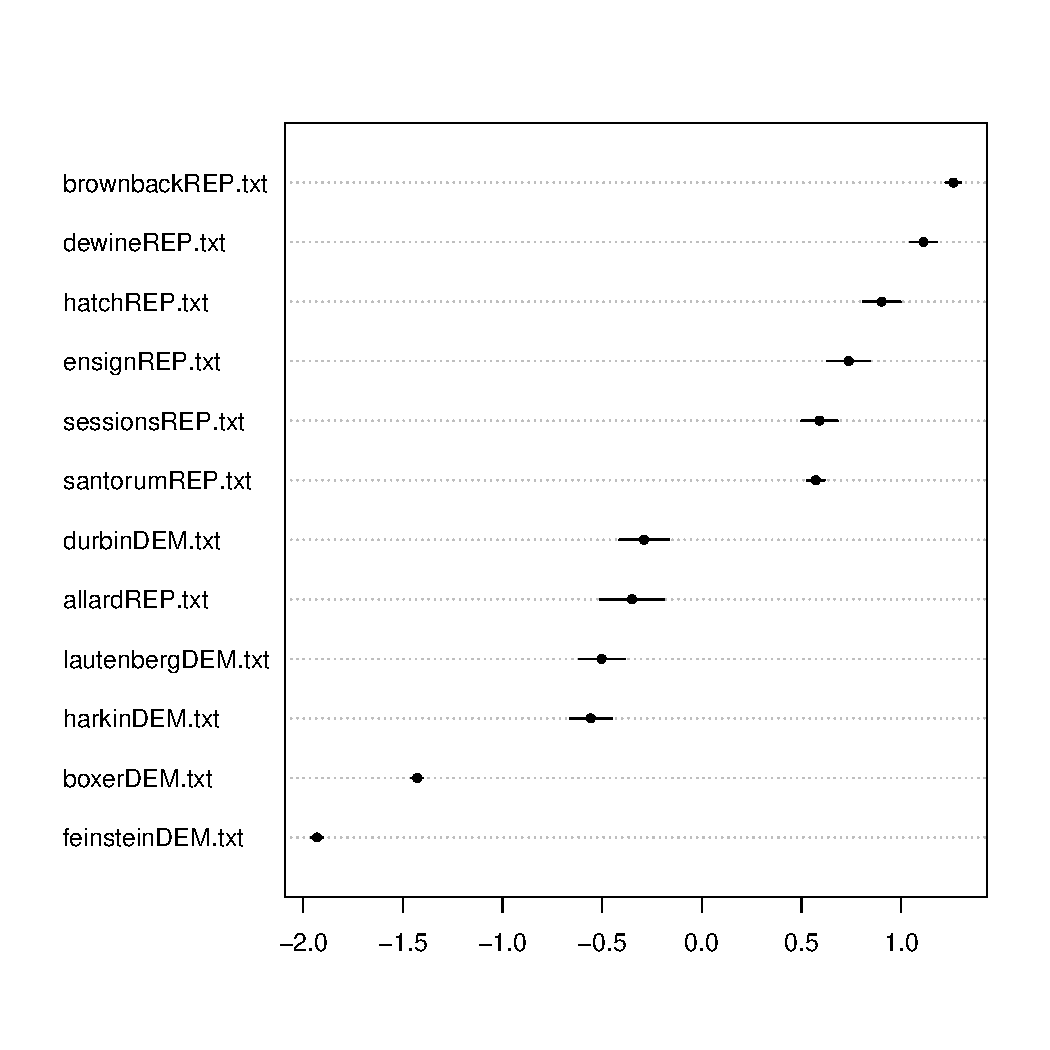
\includegraphics[width=\maxwidth]{figure/plot-words-1} 

\end{knitrout}
\caption{A chart of speaker positions, with uncertainty.}
\label{senplot}
\end{center}
\end{figure}

The analysis suggests that there is a partisan divide, with Democrats having position estimates that are smaller than Republicans. Let's take a look at the word estimates and see how they line up on the dimension. Let's plot the slope estimates for some likely looking word stems.  But first we have to extract them from all the other parameters.
\begin{knitrout}
\definecolor{shadecolor}{rgb}{0.969, 0.969, 0.969}\color{fgcolor}\begin{kframe}
\begin{alltt}
\hlstd{word.coefs} \hlkwb{<-} \hlkwd{coef}\hlstd{(senate.res,} \hlstr{'poisson'}\hlstd{)}\hlopt{$}\hlstd{words} \hlcom{## just take the word parameters}
\hlstd{wds} \hlkwb{<-} \hlkwd{c}\hlstd{(}\hlstr{"life"}\hlstd{,}\hlstr{"unborn"}\hlstd{,} \hlstr{"choic"}\hlstd{,}\hlstr{"her"}\hlstd{,}\hlstr{"woman"}\hlstd{,}\hlstr{"health"}\hlstd{,}\hlstr{"born"}\hlstd{,}\hlstr{"babi"}\hlstd{,}\hlstr{"defenseless"}\hlstd{,}\hlstr{"gruesom"}\hlstd{,}\hlstr{"kill"}\hlstd{)}
\hlstd{word.coefs[wds,]}
\end{alltt}
\begin{verbatim}
                  beta        psi
life        -0.2930615  2.1350161
unborn       0.3706191 -0.9095174
choic       -0.7901168  0.5999905
her         -0.5903537  1.8643746
woman       -1.1258828  1.2423738
health      -1.0917917  2.3641468
born         0.3985378  0.8163271
babi         0.5370816  1.9659210
defenseless  2.5680198 -4.2917566
gruesom      1.1676885 -1.0422918
kill         0.1140630  1.1792684
\end{verbatim}
\end{kframe}
\end{knitrout}
Do the estimates make sense?  Again, it's easier to see if we plot them, as in Fig.~\ref{wds}.

\begin{figure}[htbp]
\begin{center}
\begin{knitrout}
\definecolor{shadecolor}{rgb}{0.969, 0.969, 0.969}\color{fgcolor}\begin{kframe}
\begin{alltt}
\hlkwd{dotchart}\hlstd{(word.coefs[wds,} \hlstr{'beta'}\hlstd{], wds)}
\end{alltt}
\end{kframe}
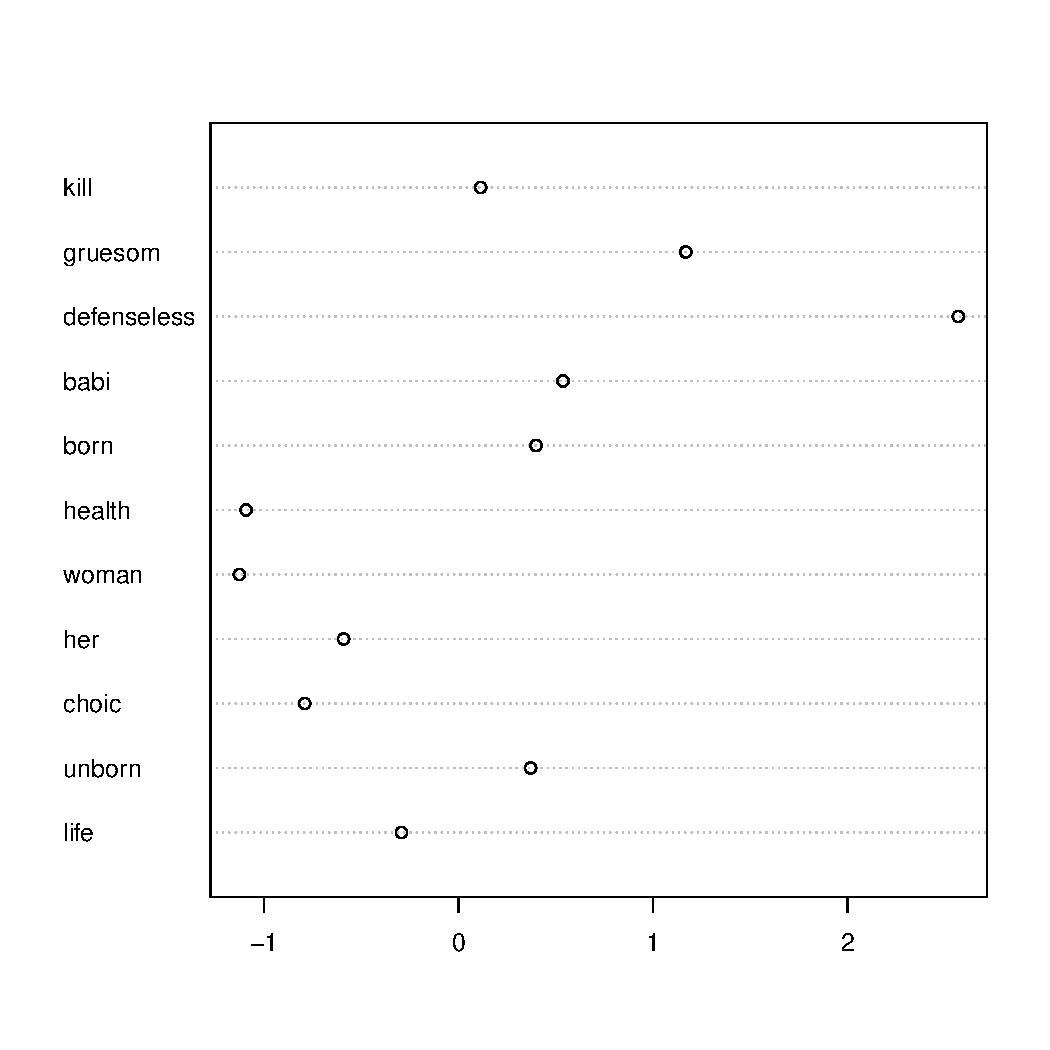
\includegraphics[width=\maxwidth]{figure/plot-words-again-1} 

\end{knitrout}
\caption{A chart of word slopes (sensitivity to ideological position) for the word stems.}
\label{wds}
\end{center}
\end{figure}

If we were being thorough about these words we'd check they do what we think they do by looking 
at them in context.

% We first construct a term-document matrix out of the speeches. We do this using the open-source program \texttt{JFreq}. The program allows us to perform some standard preprocessing of the texts prior to constructing the word frequency dataset. Drag and drop the speech text files into the window. Check the boxes \textit{lowercase}, \textit{no numbers}, \textit{no currency}, and \textit{stemmer} (choosing \textit{English}). The last option applies an algorithm that reduces inflected words to their root (stem), meaning that words like ``language'' and ``languages'' are counted as the same word and not twice (note the obvious caveat of such a procedure). 

% Save the term document matrix as a ``csv'' file.  


\end{document}
